\section[Die Architektur der Applikation(Jürgen Hetzel)]{Die Architektur der Applikation
\begin{tiny} (Jürgen Hetzel)\end{tiny}}

\begin{figure}[H]
\centering
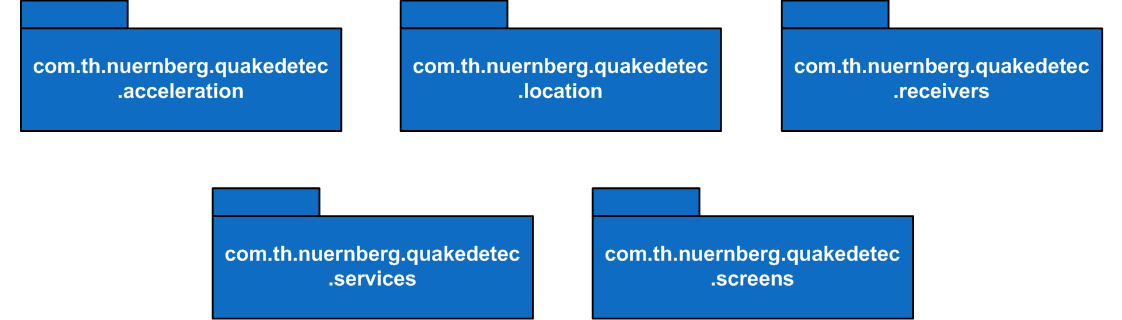
\includegraphics[width=\textwidth]{/java_pakete.png}
\caption{Die Pakete der Applikation}
\label{fig:java_pakages}
\end{figure}
Der Code der Applikation unterteilt sich in fünf Pakete, mit unterschiedlichen Aufgabenbereichen.
Nachfolgend wird ein Überblick über diese gegeben. In den zugehörigen Klassendiagrammen werden
neuerstellte Klassen mit orangenen und die des Android-Frameworks mit blauen Hintergrund
dargestellt. Die detaillierte Beschreibung erfolgt in den späteren Abschnitten der Dokumenation.

\subsection{Die Klassen des Pakets acceleration}
\begin{figure}[H]
\centering
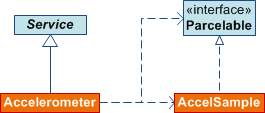
\includegraphics{/classdiagramm_acceleration.png}
\caption{Klassendiagramm von .acceleration}
\label{fig:classdiagramm_acceleration}
\end{figure}
Mit Hilfe eines \emph{SensorListener} erfährt das Objekt der Klasse \emph{Accelerometer} von
Beschleunigungsänderungen am Sensor. Anschließend sendet es ein Beschleunigungs-Muster, welches
durch \emph{AccelSample} repräsentiert wird, systemweit per \emph{Broadcast}. Dast Interface
\emph{Parcelable} dient hierbei der Serialisierung.


\subsection{Die Klassen des Pakets location}
\begin{figure}[H]
\centering
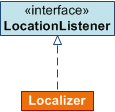
\includegraphics{/classdiagramm_location.png}
\caption{Klassendiagramm von .location}
\label{fig:classdiagramm_location}
\end{figure}
Dieses Paket beherbergt lediglich die Klasse \emph{Localizer}. Sie implementiert einen
\emph{LocationListener} und übernimmt die Bestimmung der Standortdaten.



\subsection{Die Klassen des Pakets receivers}
\begin{figure}[H]
\centering
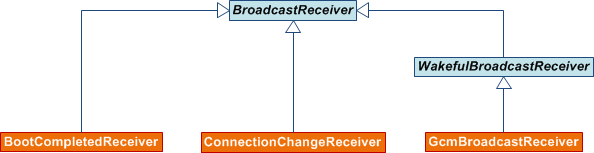
\includegraphics[width=\textwidth]{/classdiagramm_receivers.png}
\caption{Klassendiagramm von .receivers}
\label{fig:classdiagramm_receivers}
\end{figure}

In diesem Paket wird das Handling der \emph{Broadcasts} durchgeführt.
Erhält \emph{BootCompletedReceiver} eine Nachricht bezüglich des vollendetenden
Bootvorgangs, startet dieser den \emph{BackgroundService} der Applikation. 
Zumal die App auf eine Internetverbindung angewiesen ist, reagiert der
\emph{ConnectionChangeReceiver} auf eine Änderung der Konnektivität. Der \emph{GcmBroadCastReceiver}
kümmert sich um empfangene \emph{Google Cloud Messaging Nachrichten}. Mittels Ableitung von
der abstrakten Klasse \emph{WakefulBroadcastReceiver} ist es ihm möglich, die CPU solange vom
Standby-Modus abzuhalten, bis der zugehörige Service gestartet wurde.


\subsection{Die Klassen des Pakets services}
\begin{figure}[H]
\centering
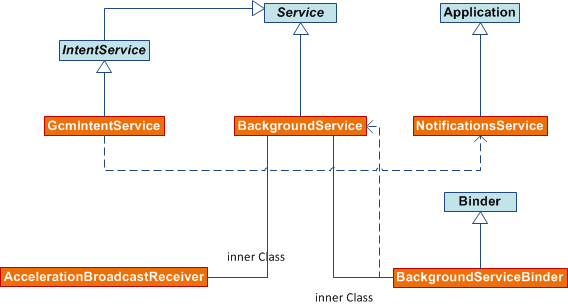
\includegraphics{/classdiagramm_services.png}
\caption{Klassendiagramm von .services}
\label{fig:classdiagramm_services}
\end{figure}

Der \emph{BackgroundService} wird nach Booten des Geräts gestartet und läuft
fortwährend im Hintergrund. Er registriert das Android-Gerät mit Positionsangabe beim Server
und trägt die Verantwortung der Erdbebenauswertung. Falls ein Erdbeben erkannt wird,
schickt er eine entsprechende Nachricht an den Server. Der GcmIntentService übernimmt die
Handhabung der \emph{Google Cloud Messaging Nachrichten}. Er ist von
\emph{IntentService} abgeleitet und läuft als eigener Worker-Thread, der die Anfragen in Form einer
Queue ablegt und abarbeitet \cite[vgl.][]{ADevIntentService}. Bei \emph{NotificationsService}
handelt es sich um keinen Android-Baustein \emph{Service}. Er erstellt Benachrichtigungen nach
bestimmter Konfiguration und befindet sich lediglich auf Grund seiner Aufgaben in diesem Paket.
Mittels der Ableitung von \emph{Binder} der inneren Klasse \emph{BackgroundServiceBinder}, wird eine
Schnittstelle zur Kommunikation mit den Service-Nutzern bereitgestellt \cite[vgl.][S. 174]{AppsProg}.


\subsection{Die Klassen des Pakets screens}
\begin{figure}[H]
\centering
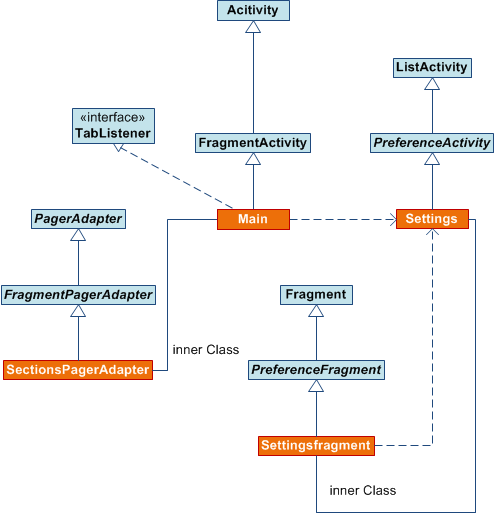
\includegraphics{/classdiagramm_activities.png}
\caption{Klassendiagramm der Activities}
\label{fig:classdiagramm_activities}
\end{figure}
Dieses Paket repräsentiert den eigentlichen Bildschirminhalt Die Ableitung von
\emph{FragementsPagerAdapter} schafft die Voraussetzung, um durch die Inhalte der App
blättern zu können. Das Interface \emph{TabListener} lieftert die für die Reiter
notwendigen Callback-Methoden . \emph{PreferenceActivity} stellt die Oberklasse für
Settings-Activities seit Android 3.0 dar \cite[vgl.][]{ADevPrefActivity}. Settings bietet diverse
Einstellungen, wie etwa bezüglich der Kartenansicht (Kartenart), Server und Benachrichtigungen. Fragmente ermöglichen einen
modularen Aufbau der Activities. Die \emph{Main-Activity} beherbergt die Fragmente \emph{Info}
und \emph{DeviceMap}, die in nachfolgenden Klassendiagramm dargestellt sind.


\begin{figure}[H]
\centering
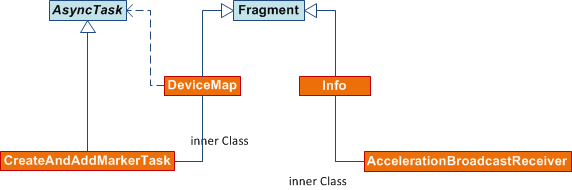
\includegraphics{/classdiagramm_fragments.png}
\caption{Klassendiagramm der Fragmente}
\label{fig:classdiagramm_fragments}
\end{figure}
Das Fragment \emph{DeviceMap} stellt die Karte mit Positionsmarkierungen dar.  
Mittels Ableitung von \emph{AsyncTask} können Operationen im Hintergrund durchgeführt werden und
ihre Ergebenisse ins {User Interface} einfließen \cite[vgl.][]{ADevAsyncTask}. Durch das Fragment
\emph{Info} wird die graphische Darstellung der Beschleunigungssensordaten und Informationen wie beispielsweise der Anzahl der
verbundenen Geräten realisiert.





